\documentclass{article}
\iffalse
This file is protected by Copyright. Please refer to the COPYRIGHT file
distributed with this source distribution.

This file is part of OpenCPI <http://www.opencpi.org>

OpenCPI is free software: you can redistribute it and/or modify it under the
terms of the GNU Lesser General Public License as published by the Free Software
Foundation, either version 3 of the License, or (at your option) any later
version.

OpenCPI is distributed in the hope that it will be useful, but WITHOUT ANY
WARRANTY; without even the implied warranty of MERCHANTABILITY or FITNESS FOR A
PARTICULAR PURPOSE. See the GNU Lesser General Public License for more details.

You should have received a copy of the GNU Lesser General Public License along
with this program. If not, see <http://www.gnu.org/licenses/>.
\fi

\author{} % Force author to be blank
%----------------------------------------------------------------------------------------
% Paper size, orientation and margins
%----------------------------------------------------------------------------------------
\usepackage{geometry}
\geometry{
	letterpaper,			% paper type
	portrait,				% text direction
	left=.75in,				% left margin
	top=.75in,				% top margin
	right=.75in,			% right margin
	bottom=.75in			% bottom margin
 }
%----------------------------------------------------------------------------------------
% Header/Footer
%----------------------------------------------------------------------------------------
\usepackage{fancyhdr} \pagestyle{fancy} % required for fancy headers
\renewcommand{\headrulewidth}{0.5pt}
\renewcommand{\footrulewidth}{0.5pt}
\rhead{\small{ANGRYVIPER Team}}
%----------------------------------------------------------------------------------------
% Appendix packages
%----------------------------------------------------------------------------------------
\usepackage[toc,page]{appendix}
%----------------------------------------------------------------------------------------
% Defined Commands & Renamed Commands
%----------------------------------------------------------------------------------------
\renewcommand{\contentsname}{Table of Contents}
\renewcommand{\listfigurename}{List of Figures}
\renewcommand{\listtablename}{List of Tables}
\newcommand{\todo}[1]{\textcolor{red}{TODO: #1}\PackageWarning{TODO:}{#1}} % To do notes
\newcommand{\code}[1]{\texttt{#1}} % For inline code snippet or command line
%----------------------------------------------------------------------------------------
% Various pacakges
%----------------------------------------------------------------------------------------
\usepackage{hyperref} % for linking urls and lists
\usepackage{graphicx} % for including pictures by file
\usepackage{listings} % for coding language styles
\usepackage{rotating} % for sideways table
\usepackage{pifont}   % for sideways table
\usepackage{pdflscape} % for landscape view
%----------------------------------------------------------------------------------------
% Table packages
%----------------------------------------------------------------------------------------
\usepackage{tabularx} % c=center,l=left,r=right,X=fill
\usepackage{float}
\floatstyle{plaintop}
\usepackage[tableposition=top]{caption}
\newcolumntype{P}[1]{>{\centering\arraybackslash}p{#1}}
\newcolumntype{M}[1]{>{\centering\arraybackslash}m{#1}}
%----------------------------------------------------------------------------------------
% Block Diagram / FSM Drawings
%----------------------------------------------------------------------------------------
\usepackage{tikz}
\usetikzlibrary{shapes,arrows,fit,positioning}
\usetikzlibrary{automata} % used for the fsm
%----------------------------------------------------------------------------------------
% Colors Used
%----------------------------------------------------------------------------------------
\usepackage{colortbl}
\definecolor{blue}{rgb}{.7,.8,.9}
\definecolor{ceruleanblue}{rgb}{0.16, 0.32, 0.75}
\definecolor{drkgreen}{rgb}{0,0.6,0}
\definecolor{deepmagenta}{rgb}{0.8, 0.0, 0.8}
\definecolor{cyan}{rgb}{0.0,0.6,0.6}
\definecolor{maroon}{rgb}{0.5,0,0}
%----------------------------------------------------------------------------------------
% Update the docTitle and docVersion per document
%----------------------------------------------------------------------------------------
\def\docTitle{Component Data Sheet}
\def\docVersion{1.3}
%----------------------------------------------------------------------------------------
\date{Version \docVersion} % Force date to be blank and override date with version
\title{\docTitle}
\lhead{\small{\docTitle}}

\def\comp{cic\_int}
\edef\ecomp{cic_int}
\def\Comp{CIC Interpolator}
\graphicspath{ {figures/} }

\begin{document}

\section*{Summary - \Comp}
\begin{tabular}{|c|M{13.5cm}|}
	\hline
	\rowcolor{blue}
	                  &                                                    \\
	\hline
	Name              & \comp                                              \\
	\hline
	Worker Type       & Application                                        \\
	\hline
	Version           & v\docVersion \\
	\hline
	Release Date      & February 2018 \\
	\hline
	Component Library & ocpi.assets.dsp\_comps                              \\
	\hline
	Workers           & \comp.hdl                                          \\
	\hline
	Tested Platforms  & xsim, isim, modelsim, alst4, ml605, ZedBoard(PL), Matchstiq-Z1(PL) \\
	\hline
\end{tabular}

\section*{Functionality}
\begin{flushleft}
	The CIC interpolator has \verb+N+ cascaded comb stages with an input data rate of $\frac{f_{s}}{R}$, followed by a rate change by a factor \verb+R+, followed by \verb+N+ cascaded integrator stages with an output data rate of $f_{s}$. The differential delay, \verb+M+, affects the slope of the transition region. Figure \ref{fig:cic} diagrams the interpolating CIC filter.

	\begin{figure}[ht]
		\centering
		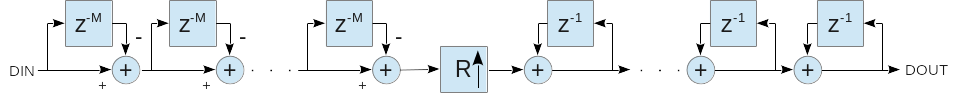
\includegraphics[scale=.6]{cic_interpolator_block_diagram}
		\caption{Cascaded Integration Comb Decimation filter Block Diagram}
		\label{fig:cic}
	\end{figure}
\end{flushleft}

\section*{Worker Implementation Details}
\subsection*{\comp.hdl}
\subsubsection*{Number of Stages}
\begin{flushleft}
	The generic \verb+N+ sets the number of integrators and comb stages in the filter.	Increasing the number of stages increases the attenuation in the sidelobes, as well as the bandwidth of the passband. The recommended range for this parameter is 3 to 6. Consult the reference material for an in depth discussion of the frequency response of the filter as a function of the generics in this module.
\end{flushleft}
\subsubsection*{Bit Growth}
\begin{flushleft}
	For this design, the output data width for the comb stages is configurable via	\verb+ACC_WIDTH+. To adjust for bit growth in the data path and to ensure no quantization error at the output, this equation should be used to determine the value of \verb+ACC_WIDTH+.

	\begin{equation} \label{eq:acc_width}
		ACC\_WIDTH = N*CEIL(log_2(R*M))+DIN\_WIDTH
	\end{equation}
\end{flushleft}

\section*{Theory}
\begin{flushleft}
	A CIC filter is comprised of \verb+N+ integrator sections cascaded together with \verb+N+ comb sections. Combining the transfer functions for the two sections, we arrive at the system response function seen in Equation 1.

	\begin{equation} \label{eq:response_function}
		H(z) = [H_{int}(z)]^N[H_{comb}(z)]^N = \frac{1}{(1-z^{-1})^N}(1-z^{-R+M})^N = 	\frac{(1 - z^{-R+M})^N}{(1-z^{-1})^N}
	\end{equation}

	The magnitude response of the CIC filter is low pass with nulls at multiples of $f=\frac{1}{RM}$. The region surrounding the nulls is where aliasing occurs, so 	this aliasing effect must be considering when choosing \verb+N+, \verb+M+, and \verb+R+.
\end{flushleft}

\section*{Block Diagrams}
\subsection*{Top level}
\begin{center}
	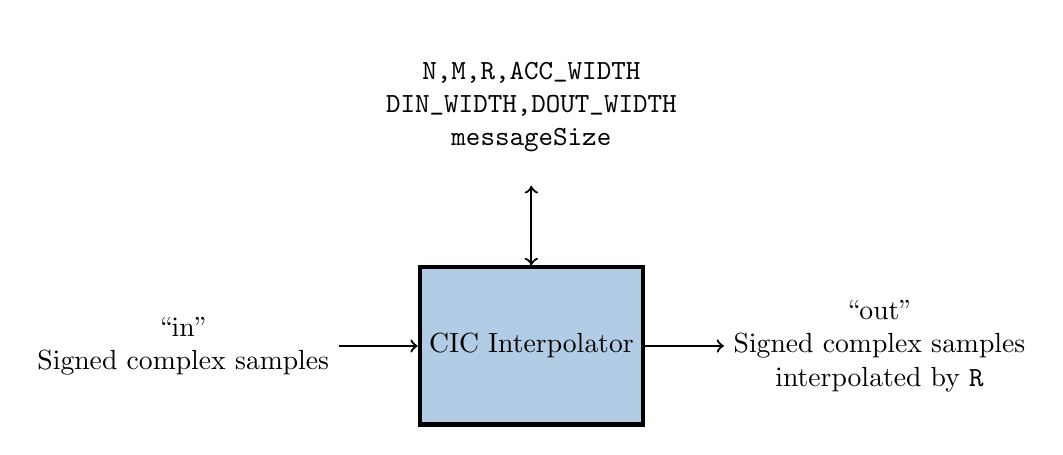
\begin{tikzpicture}[% List of styles applied to all, to override specify on a case-by-case
			every node/.style={
				align=center,  		% use this so that the "\\" for line break works
				minimum size=2cm	% creates space above and below text in rectangle
			},
			every edge/.style={draw,thick}
		]
		\node[rectangle,ultra thick,draw=black,fill=blue](R2){\Comp};
		\node[rectangle,draw=white,fill=white](R3)[left= of R2]{``in'' \\ Signed complex samples};
		\node[rectangle,draw=white,fill=white](R4)[right= of R2]{``out'' \\ Signed complex samples \\ interpolated by \verb+R+};
		\node[rectangle,draw=white,fill=white](R5)[above= of R2]{\verb+N,M,R,ACC_WIDTH+ \\ \verb+DIN_WIDTH,DOUT_WIDTH+ \\ \verb+messageSize+};
		\path[->]
		(R3)edge []	node [] {} (R2)
		(R2)edge []	node [] {} (R4)
		(R2)edge []	node [] {} (R5)
		(R5)edge []	node [] {} (R2)
		;
	\end{tikzpicture}
	\captionof{figure}{Top Level Block Diagram}
\end{center}
\newpage
\subsection*{State Machine}
\begin{flushleft}
	Only one finite-state machine (FSM) is implemented by this worker. The FSM supports Zero-Length Messages.
\end{flushleft}
{\centering\captionsetup{type=figure}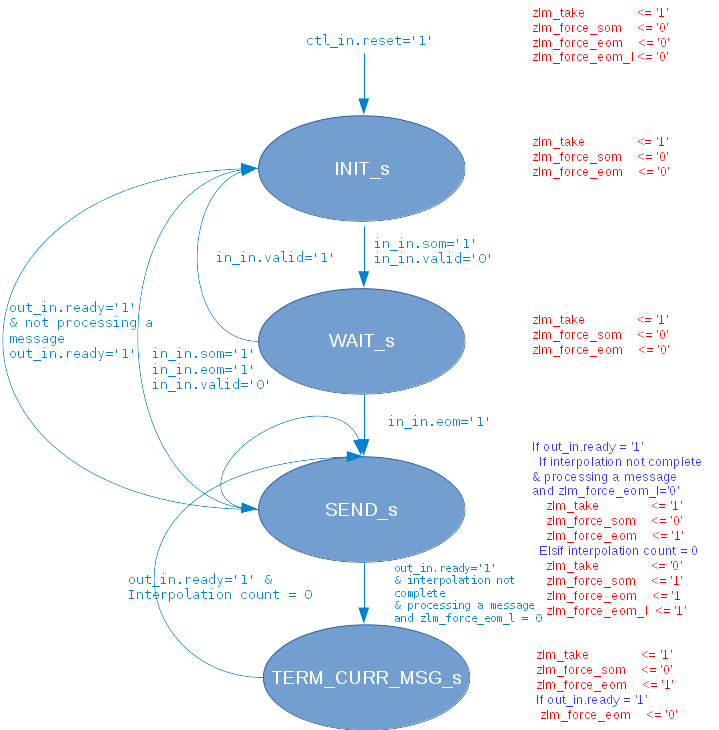
\includegraphics[scale=0.45]{cic_interpolator_zlm_fsm}
	\captionof{figure}{Zero-Length Message FSM}
	\label{fig:zlm_fsm}}

\newpage

\section*{Source Dependencies}
\subsection*{\comp.hdl}
\begin{itemize}
	\item ocpiassets/components/dsp\_comps/cic\_int.hdl/cic\_int.vhd
	\item ocpiassets/hdl/primitives/dsp\_prims/dsp\_prims\_pkg.vhd
	      \subitem ocpiassets/hdl/primitives/dsp\_prims/cic/src/cic\_int\_gen.vhd
\end{itemize}

\begin{landscape}
	\section*{Component Spec Properties}
	\begin{scriptsize}
		\begin{tabular}{|p{3cm}|p{1.5cm}|c|c|c|c|c|p{7cm}|}
			\hline
			\rowcolor{blue}
			Name                      & Type   & SequenceLength & ArrayDimensions & Accessibility      & Valid Range & Default & Usage                                            \\
			\hline \verb+N+           & UChar  & -              & -               & Readable           & -           & -       & Number of Stages                                 \\
			\hline \verb+M+           & UChar  & -              & -               & Readable           & -           & -       & Differential Delay                               \\
			\hline \verb+R+           & UShort & -              & -               & Readable           & -           & -       & Interpolation Factor                             \\
			\hline \verb+ACC_WIDTH+   & UChar  & -              & -               & Readable           & -           & -       & Accumulation Width *(\ref{eq:response_function}) \\
			\hline \verb+DIN_WIDTH+   & UChar  & -              & -               & Readable           & -           & -       & Input data width                                 \\
			\hline \verb+DOUT_WIDTH+  & UChar  & -              & -               & Readable           & -           & -       & Output data width                                \\
			\hline \verb+messageSize+ & UShort & -              & -               & Readable, Writable & -           & 8192    & Number of bytes in output message                \\
			\hline
		\end{tabular}
	\end{scriptsize}
	\section*{Worker Properties}

	\subsection*{\comp.hdl}
	\begin{scriptsize}
		\begin{tabular}{|c|p{2cm}|p{1cm}|c|c|c|p{2cm}|p{1cm}|p{5cm}|}
			\hline
			\rowcolor{blue}
			Type         & Name              & Type & SequenceLength & ArrayDimensions & Accessibility & Valid Range & Default & Usage                                            \\
			\hline
			SpecProperty & \verb+N+          & -    & -              & -               & Parameter     & 3-6         & 3       & Number of Stages                                 \\
			\hline
			SpecProperty & \verb+M+          & -    & -              & -               & Parameter     & 1-2         & 1       & Differential Delay                               \\
			\hline
			SpecProperty & \verb+R+          & -    & -              & -               & Parameter     & 4-8192      & 4       & Decimation Factor                                \\
			\hline
			SpecProperty & \verb+DIN_WIDTH+  & -    & -              & -               & Parameter     & 16          & 16      & Input Data Width                                 \\
			\hline
			SpecProperty & \verb+ACC_WIDTH+  & -    & -              & -               & Parameter     & *           & 22      & Accumulation Width *(\ref{eq:response_function}) \\
			\hline
			SpecProperty & \verb+DOUT_WIDTH+  & -    & -              & -               & Parameter           & 16          & 16      & Output Data Width                                \\
			\hline
			Property     & \verb+CHIPSCOPE_p+ & Bool & -              & -               & Readable, Parameter & Standard    & false   & Include ChipScope circuit                        \\
			\hline
		\end{tabular}
	\end{scriptsize}

	\section*{Component Ports}
	\begin{scriptsize}
		\begin{tabular}{|M{2cm}|M{1.5cm}|M{4cm}|c|c|M{9cm}|}
			\hline
			\rowcolor{blue}
			Name & Producer & Protocol           & Optional & Advanced & Usage                  \\
			\hline
			in   & false    & iqstream\_protocol & false    & -        & Signed complex samples \\
			\hline
			out  & true     & iqstream\_protocol & false    & -        & Signed complex samples \\
			\hline
		\end{tabular}
	\end{scriptsize}
	\section*{Worker Interfaces}
	\subsection*{\comp.hdl}
	\begin{scriptsize}
		\begin{tabular}{|M{2cm}|M{1.5cm}|c|c|M{12cm}|}
			\hline
			\rowcolor{blue}
			Type            & Name & DataWidth & Advanced                & Usage                  \\
			\hline
			StreamInterface & in   & 32        & ZeroLengthMessages=true & Signed complex samples \\
			\hline
			StreamInterface & out  & 32        & ZeroLengthMessages=true & Signed complex samples \\
			\hline
		\end{tabular}
	\end{scriptsize}
\end{landscape}

\section*{Control Timing and Signals}
\begin{flushleft}
	The CIC Interpolation filter HDL worker uses the clock from the Control Plane and standard Control Plane signals.\medskip

	%\noindent This worker has an processing group delay of (N*R*M + R*2 + 2) valid input data cycles. After this initial delay, valid output data is given N*2+1 clock cycles after input data is taken.\par\bigskip

	This worker has a latency of \verb+N+*2+1 valid input data clock cycles.\medskip

	\begin{tabular}{|M{4.5cm}|M{4.5cm}|M{1cm}|M{1.5cm}|M{2cm}|M{1cm}|M{1cm}|M{2.5cm}|}
		\hline
		\rowcolor{blue}
		\hline
		Latency         \\
		\hline
		\verb+N+*2+1    \\
		\hline
	\end{tabular}
\end{flushleft}

\section*{Performance and Resource Utilization}
\subsection*{\comp.hdl}
\input{../../\ecomp.hdl/utilization.inc}
\newpage
\section*{Test and Verification}
Two test cases are implemented to validate the CIC Interpolator component:

\begin{enumerate}
	\item Unity gain response to DC: The CIC Interpolator gain is calculated using the following equation:
	      \begin{equation} \label{eq:cic_gain}
	      	CIC\ Gain = \frac{(R*M)^N}{2^{CEIL(N*log_2(R*M))}}
	      \end{equation}
	\item Tone waveform: A waveform containing a tone at 50 Hz is sampled at 1024000/R and processed by the worker. The output data (interpolated waveform) is checked to ensure the 50 Hz tone is present.
\end{enumerate}\medskip

For the plots below, a CIC Interpolator with the following parameter set was used: \verb+N+=3, \verb+M+=1, \verb+R+=2048, and \verb+ACC_WIDTH+=49.\bigskip

\newpage
	For Case \#1, the plots below show the input with the I-leg zoomed in the show the amplitude is 32767, and output data with the I-leg zoomed to show an amplitude of 32767, which can be calculated using \ref{eq:cic_gain}, shown below, and the Q-leg showing the worker delay before reaching it steady-state value.
		  \begin{equation} \label{eq:cic_gain_applied}
	      	Output Amplitude = 32767*\frac{(2048*1)^3}{2^{CEIL(3*log_2(2038*1))}} = 32767*1=32767
	      \end{equation}

	\begin{figure}[ht]
		\centering
		\begin{minipage}{.5\textwidth}
			\centering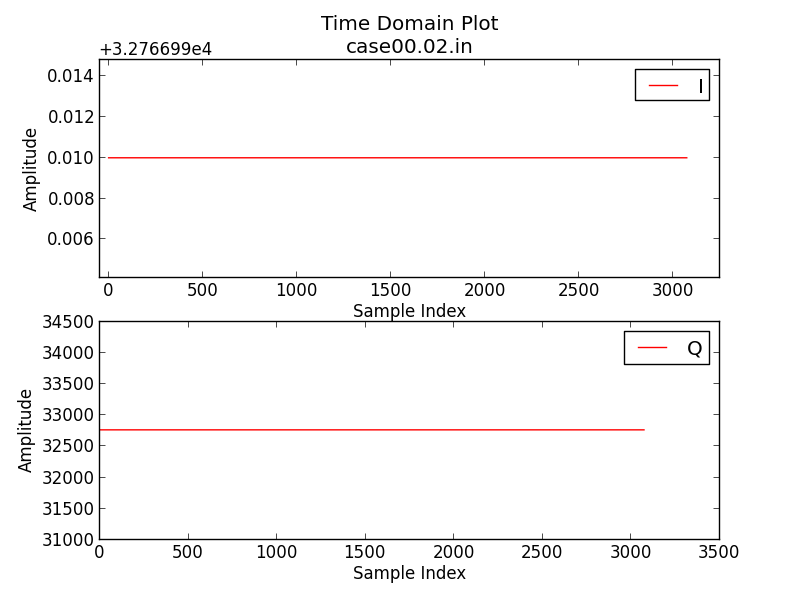
\includegraphics[width=1.0\linewidth]{input_time_DC}
			\captionof{figure}{Time Domain: DC with amp=32767}
			\label{fig:input_time_DC}
		\end{minipage}%
		\begin{minipage}{.5\textwidth}
			\centering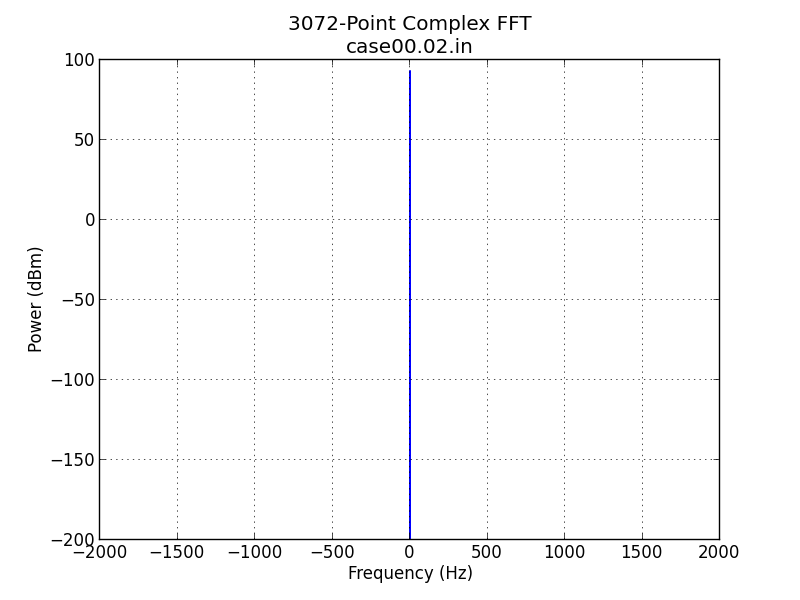
\includegraphics[width=1.0\linewidth]{input_freq_DC}
			\captionof{figure}{Frequency Domain: 0 Hz}
			\label{fig:input_freq_DC}
		\end{minipage}
	\end{figure}


	\begin{figure}[ht]
		\centering
		\begin{minipage}{.5\textwidth}
			\centering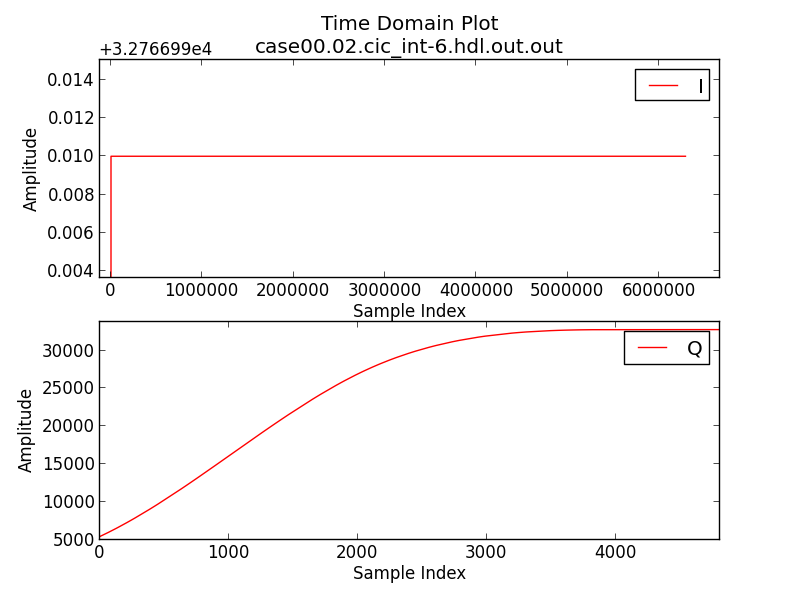
\includegraphics[width=1.0\linewidth]{output_time_DC}
			\captionof{figure}{Time Domain: DC with amp=32767}
			\label{fig:output_time_DC}
		\end{minipage}%
		\begin{minipage}{.5\textwidth}
			\centering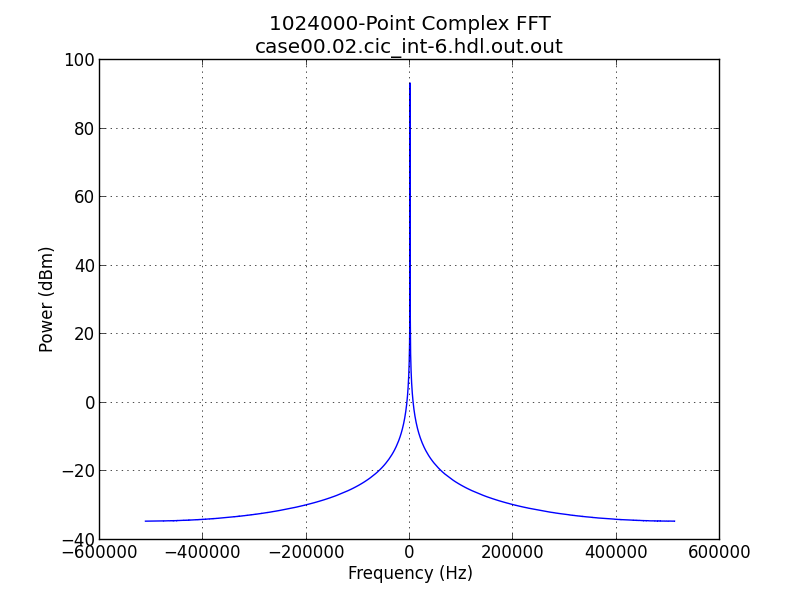
\includegraphics[width=1.0\linewidth]{output_freq_DC}
			\captionof{figure}{Frequency Domain: 0 Hz}
			\label{fig:output_freq_DC}
		\end{minipage}
	\end{figure}

\newpage
The input time-domain plot below shows the I-leg zoomed into one cycle and Q-leg showing all samples of a 50 Hz tone sampled at 1024000/R=1024000/2048=500 Hz, which results in 10 samples/cycle. The input freq-domain plot shows the generated tone at 50 Hz.
The output time-domain plot below shows the I-leg zoomed into approximately two cycles and Q-leg showing all samples of a 50 Hz tone sampled at (1024000/R)*R=(1024000/2048)*2048=1024000 Hz, which results in 20480 samples/cycle. The output freq-domain plot shows the expected tone at 50 Hz.

	\begin{figure}[ht]
		\centering
		\begin{minipage}{.5\textwidth}
			\centering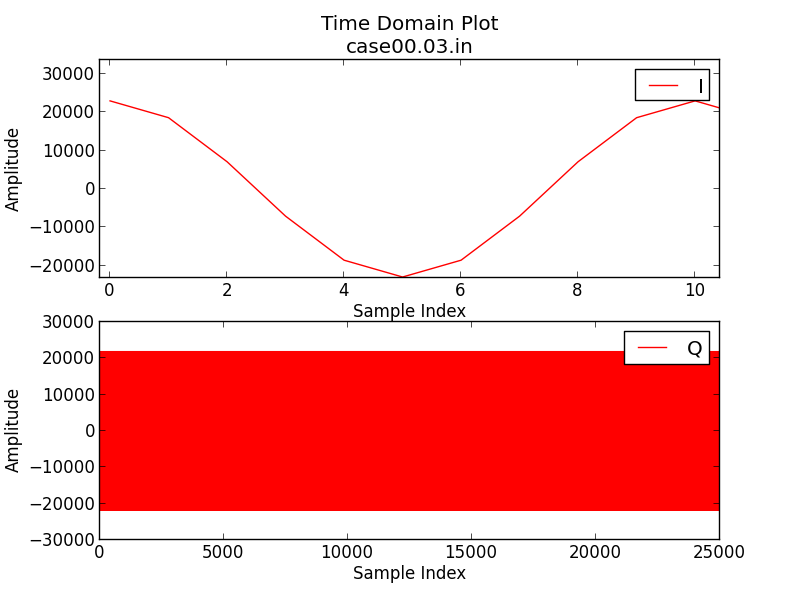
\includegraphics[width=1.0\linewidth]{input_time_R2048}
			\captionof{figure}{Time Domain}
			\label{fig:input_time_R2048}
		\end{minipage}%
		\begin{minipage}{.5\textwidth}
			\centering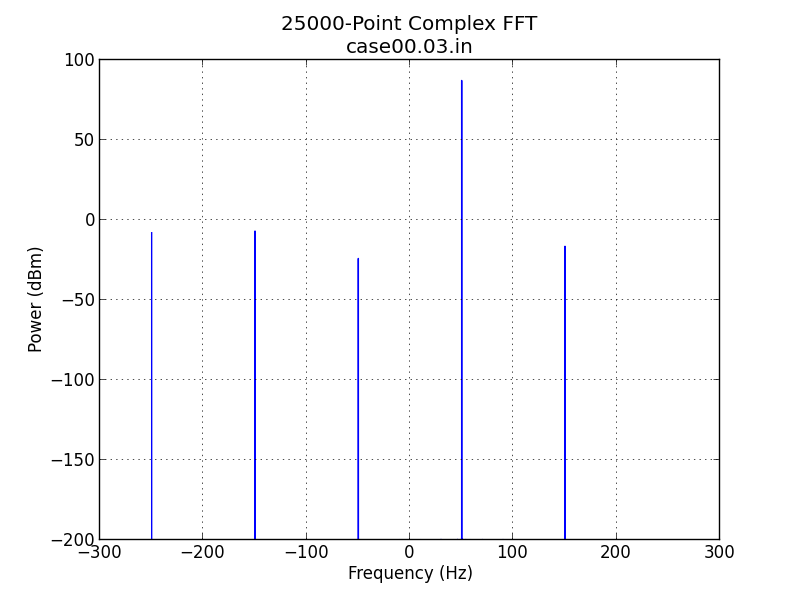
\includegraphics[width=1.0\linewidth]{input_freq_R2048}
			\captionof{figure}{Frequency Domain: 50 Hz}
			\label{fig:input_freq_R2048}
		\end{minipage}
	\end{figure}

	\begin{figure}[ht]
		\centering
		\begin{minipage}{.5\textwidth}
			\centering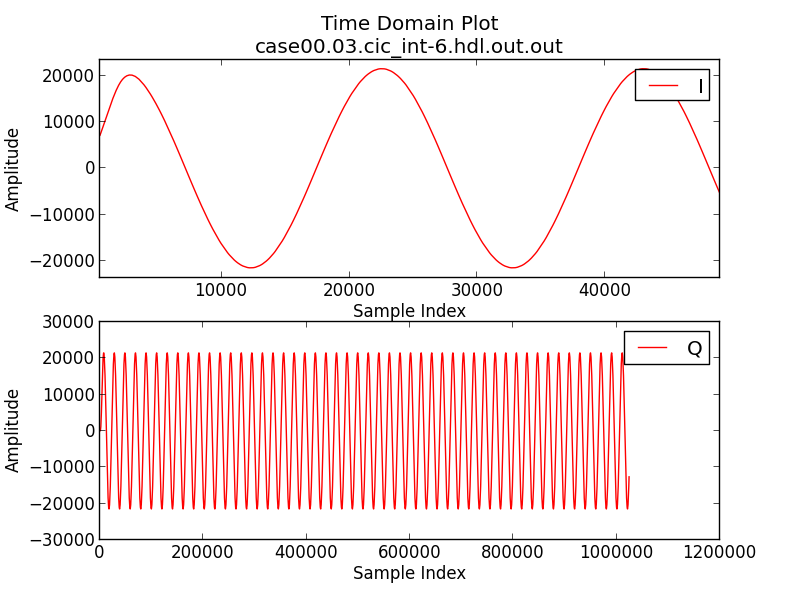
\includegraphics[width=1.0\linewidth]{output_time_R2048}
			\captionof{figure}{Time Domain}
			\label{fig:output_time_R2048}
		\end{minipage}%
		\begin{minipage}{.5\textwidth}
			\centering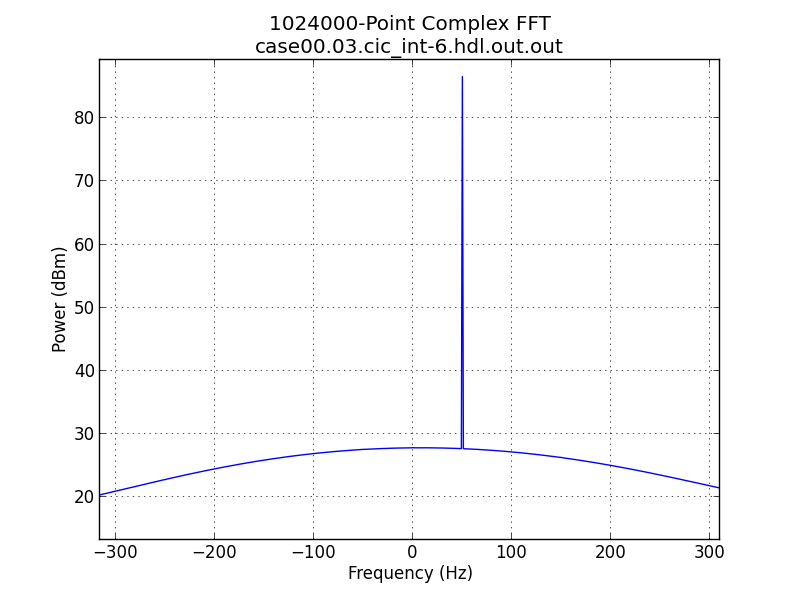
\includegraphics[width=1.0\linewidth]{output_freq_R2048}
			\captionof{figure}{Frequency Domain: 50 Hz}
			\label{fig:output_freq_R2048}
		\end{minipage}
	\end{figure}

\section*{References}
(1)	Ronald E. Crochiere and Lawrence R. Rabiner. Multirate Digital Signal Processing. Prentice-Hall Signal Processing Series. Prentice Hall, Englewood Cli\_s, 1983. \\
(2)	Eugene B. Hogenauer, An Economical Class of Digital Filters for Decimation and Interpolation, IEEE Transactions on Acoustics, Speech, and Signal Processing, Vol. ASSP-29, No. 2, April 1981.

\end{document}
